\documentclass[10pt,twocolumn]{article}
\usepackage[margin=0.72in]{geometry}
\usepackage{amsmath,amssymb,amsthm}
\usepackage{graphicx}
\usepackage{booktabs}
\usepackage{xcolor}
\usepackage{hyperref}
\usepackage{xurl}
\usepackage{microtype}
\usepackage{enumitem}

\hypersetup{
  colorlinks=true,
  linkcolor=blue!60!black,
  citecolor=green!45!black,
  urlcolor=blue!65!black
}

\newtheorem{definition}{Definition}
\newtheorem{theorem}{Theorem}
\newtheorem{proposition}{Proposition}

\title{\textbf{Constructive Algebraic, Poincar\'e, and Cartier-Residue Certificates for Permanent and Hamiltonian Cycle Circuit Lower Bounds}}
\author{Lluis Eriksson\\
\small Independent Researcher \quad(\texttt{lluis@airr.science})\\
\small \textit{Companion Verification Artifact to OpenAI Math Release (November 24, 2026)}}
\date{November 26, 2026}

\begin{document}
\maketitle

\begin{abstract}
We present \texttt{PERM-HC-LB-CERT-1.0}, an independently reproducible, zero-floating-point verification framework and constructive Lean~4.35.0 kernel auditing the core finite-dimensional algebraic, sparse-gadget, balanced-cut, nonlinear Poincar\'e, Hadamard-cone, exterior-minor, and Cartier/eigenvalue counting-contradiction mechanisms underlying OpenAI's November~24, 2026 unrefereed preprint \emph{``Circuit lower bounds for Hamiltonian cycle and the permanent''} (Theorems~1.1, 3.1, 4.2, and 12.2). Without claiming to formalize infinite-dimensional Hadamard-cone ultralimits, observable-entropy reservoir coding, or universal RAM compression end-to-end, we construct a four-mode exact verifier over $\mathbb{Z}$, $\mathbb{Q}$, and $\mathbb{F}_p$ paired with 18 constructive Lean~4 theorems (0~\texttt{sorry}, 0~custom axioms, 0~\texttt{Classical.choice}, 0~warnings). Across 16 canonical certificates (\texttt{C01}--\texttt{C16}), we certify (i)~Lemma~3.4's $3\times 3$ permanent coupling gadget over $\mathbb{Q}$ and $\mathbb{F}_7$ and Corollary~3.5 degree-$\le 3$ digraph evaluations of $\operatorname{Per}_N$, $\operatorname{Det}_N$, and $\operatorname{HC}_N$ (including characteristic-2 collapse), (ii)~Section~1.3 balanced-cut crossing ranks ($5,5,8 > q^2=4$) and Lemma~4.1/Theorem~4.2 exact Poincar\'e ratios and barycentric smoothing Eq.~(4.1) on $C_4$, $C_6$, and $Q_3$, (iii)~Section~3.2 Hadamard-cone two-supplier transport savings and Section~8--9 alternating exterior minor tensors satisfying the classical Pl\"ucker relations, and (iv)~Section~18 Cartier operator residue extraction over $\mathbb{F}_5$ and $\mathbb{F}_2$ and Section~19 Eq.~(19.1)--(19.2) finite-field eigenvalue counting contradictions. All 16 certificates, 60 unit/forgery tests, and SHA-256 manifests pass deterministically.
\end{abstract}

\section{Introduction and Scope}
Valiant's algebraic complexity classes $\mathrm{VP}$ and $\mathrm{VNP}$ place the directed Hamiltonian cycle polynomial $\operatorname{HC}_N$ (complete over every field) and the permanent $\operatorname{Per}_N$ (complete outside characteristic~2, where $\operatorname{Per}_N = \operatorname{Det}_N$~\cite{berkowitz1984computing}) at the center of algebraic circuit lower bounds~\cite{valiant1979completeness}. In its November~24, 2026 unrefereed preprint~\cite{openai2026permhc}, OpenAI proves a superpolynomial degree-component border lower bound $L^{[N]}_F(\operatorname{HC}_N) \ge \exp(c(\log N)^2/(\log\log N)^2)$ over every field (and for $\operatorname{Per}_N$ when $\operatorname{char} F \ne 2$, Theorem~1.1), already attained on degree-$\le 3$ sparse graphs (Corollary~3.5).

The proof splits every characteristic $\chi$ into two cases via Strassen's asymptotic spectrum~\cite{strassen1988asymptotic,openai2026tensorspectrum} and Mendel--Naor nonlinear Poincar\'e inequalities~\cite{mendel2014nonlinear}: (1)~when $\chi$ has no port expanders, balanced parse-tree cuts~\cite{valiant1983fast} (Lemma~3.3), barycentric walk smoothing (Lemma~4.1, Theorem~4.2), Hadamard-cone two-supplier savings (Sec.~3.2), and exterior-algebra minor tensors (Secs.~8--11) yield $\exp(\Omega((\log N)^2/(\log\log N)^2))$; (2)~when $\chi$ admits ports, tensor-network compression, the Cartier operator~\cite{cartier1957nouvelle} on border curves (Sec.~18), and an eigenvalue trace diagonalization (Sec.~19, Eq.~19.1--19.2) yield a stretched-exponential lower bound $2^{N^{\varepsilon_\chi}}$ (Theorem~12.2).

\paragraph{Honest Scope Boundary.}
This companion artifact certifies finite-dimensional algebraic gadgets, exact rational/finite-field matrix equations, Poincar\'e ratios, cone-saving witnesses, exterior minors, Cartier residues, and finite trace contradictions extracted from~\cite{openai2026permhc}. It does \emph{not} formalize infinite-dimensional Hadamard-cone ultralimits (Secs.~6--7), Shannon-entropy reservoir coding (Sec.~5), Harder--Narasimhan flag packings (Secs.~9--11), or the universal RAM simulation compiler (Secs.~13--17).

\section{Constructive Lean 4.35.0 Kernel}
The formal kernel \texttt{PermHcLbCert.lean} compiles cleanly under Lean~4.35.0 (\texttt{-j 1}) with zero \texttt{sorry}, zero custom axioms, zero warnings, and zero dependence on \texttt{Classical.choice}. Table~\ref{tab:lean} summarizes all 18 machine-checked theorems. Highlights include Theorem~2 (exact zero-axiom verification of Lemma~3.4's $3\times 3$ permanent coupling gadget cleared by~2), Theorem~3 (equivalence of length-$\le 3$ running-sum Boolean clauses), Theorem~5 (balanced parse-tree stopping gate $d \le 3r_1$), Theorem~9 (exact barycentric variance identity), Theorem~14 (exact $2\times 4$ Pl\"ucker Grassmann relation $p_{12}p_{34}-p_{13}p_{24}+p_{14}p_{23}=0$), Theorem~16 (exact modular Sec.~19 trace contradiction), and Theorem~17 (inductive list dot-product linearity).

\begin{table}[t]
\centering
\tiny
\setlength{\tabcolsep}{3pt}
\caption{The 18 constructive Lean~4.35.0 theorems in \texttt{PermHcLbCert.lean} (0~\texttt{sorry}, 0~custom axioms, 0~\texttt{Classical.choice}).}
\label{tab:lean}
\begin{tabular}{@{}cll@{}}
\toprule
\# & Theorem Identifier & Paper Reference / Invariant \\
\midrule
1 & \texttt{per2\_det2\_char2\_collapse} & Sec.~1 $\operatorname{Per}_2 - \operatorname{Det}_2 = 2bc \equiv 0\pmod 2$ \\
2 & \texttt{lemma34\_permanent\_coupling\_gadget} & Lem.~3.4 $\operatorname{per}(2A){=}8$, all four minors $0$ \\
3 & \texttt{lemma34\_running\_sum\_clause\_equiv} & Lem.~3.4 length-$\le 3$ running-sum clause \\
4 & \texttt{lemma34\_degree4\_split\_permanent} & Lem.~3.4 degree-4 vertex split invariance \\
5 & \texttt{lemma33\_balanced\_parse\_cut} & Lem.~3.3 balanced cut $3r_1 \ge d$ \\
6 & \texttt{price\_sum\_upper\_bound} & Eq.~(2.2) inductive $\sum\phi_j \le L\cdot M$ \\
7 & \texttt{cone\_inner\_product\_scaling} & Sec.~3.2 inductive $\|x\|^2{+}\|tz\|^2{-}\|x{-}tz\|^2$ \\
8 & \texttt{sec32\_star\_benchmark\_cancellation} & Eq.~(3.4) $hdF(1)$ star cancellation \\
9 & \texttt{lemma41\_barycenter\_variance\_identity} & Lem.~4.1 exact barycentric variance \\
10 & \texttt{lemma41\_averaging\_pigeonhole} & Lem.~4.1 smoothed placement $\le 2E_S$ \\
11 & \texttt{theorem42\_poincare\_half\_floor} & Thm.~4.2 $2(n-1) \ge n$ ($\beta \ge 1/2$) \\
12 & \texttt{sec5\_cat0\_exchangeable\_subadditivity} & Eq.~(5.3) CAT(0) block subadditivity \\
13 & \texttt{exterior\_minor\_alternating} & Sec.~8 alternating $2\times 2$ determinant \\
14 & \texttt{plucker\_grassmann\_identity} & Classical Pl\"ucker invariant for Sec.~8--9 \\
15 & \texttt{cartier\_residue\_index\_law} & Sec.~18 $m\in\mathbb{Z}$ ($m{=}-1$) residue law \\
16 & \texttt{sec19\_counting\_diagonal\_contradiction} & Eq.~(19.1)--(19.2) $\Omega(H^*)\not\equiv 0$ clash \\
17 & \texttt{intDot\_add\_right} & Sec.~19 inductive dot-product linearity \\
18 & \texttt{homogeneous\_isolation\_nontrivial\_size} & Sec.~3.3/19 isolation size $s\ge 1$ \\
\bottomrule
\end{tabular}
\end{table}

\section{The \texttt{PERM-HC-LB-CERT-1.0} Protocol}
{\raggedright
Our Python verifier (\texttt{src/perm\_hc\_verifier.py}) enforces zero floating-point literals, zero \texttt{float()} calls, zero true-division operators (\texttt{/}, \texttt{/=}), zero \texttt{math} imports, \texttt{MAX\_JSON\_BYTES = 1\_000\_000}, duplicate-key rejection via \texttt{object\_pairs\_hook}, and lowest-terms rationals $[p,q]$ ($|p|,q \le 10^{12}$, $\gcd(|p|,q)=1$).

\begin{definition}[\texttt{PERM-HC-LB-CERT-1.0} Modes]
Each certificate invokes one of four exact verification modes:
\begin{enumerate}[leftmargin=*,itemsep=1.5pt,topsep=2pt]
\item \texttt{sparse\_gadgets\_and\_\allowbreak per\_hc\_det} (Sec.~1, Lem.~3.4, Cor.~3.5): When $\operatorname{char}=p>0$, every matrix entry is first validated for $p \nmid q$ and reduced entrywise into $\mathbb{F}_p$ before degree checks or polynomial evaluation (ruling out $1/p$ pole cancellation). (a)~\texttt{lemma34\_coupling\_gadget} requires $\operatorname{char}\ne 2$ and verifies $\operatorname{per}(A)=1$, all four $2\times 2$ sub-permanents deleting $(r,c)\in\{0,1\}^2$ vanish, and $A_{33}=1$; (b)~\texttt{sparse\_per\_det\_hc} rejects all-zero matrices, enforces indegree/outdegree $\le d_{\max}$ in the active field, and evaluates $\operatorname{Per}_N(X)$, $\operatorname{Det}_N(X)$, and $\operatorname{HC}_N(X)$ by exact cycle-cover enumeration, enforcing $\operatorname{Per}_N = \operatorname{Det}_N$ in characteristic~2.
\item \texttt{balanced\_cut\_and\_\allowbreak poincare} (Sec.~1.3, Lem.~3.3, 4.1, Thm.~4.2): (a)~\texttt{four\_row\_balanced\_cut\_rank} constructs $T_1+T_2 = E_{12}(q)\otimes E_{34}(q) + E_{13}(q)\otimes E_{24}(q)$ ($q\in\{2,3\}$) on disjoint local supports and verifies exact $\mathbb{Q}$-flattening ranks across all three $2\mid 2$ balanced cuts; (b)~\texttt{poincare\_and\_barycentric\_smoothing} checks $d$-regularity and symmetry of $P$, computes exact $E_P(x)$, $V_\pi(x)$, and $\beta=V_\pi/E_P$, builds $A=\frac{1}{2}(I+P)$ and $S=\frac{1}{t}\sum_{h=1}^t A^h$ (even $t$), iterates exact barycenters $x^{(g+1)}_i=\sum_j A_{ij}x^{(g)}_j$, and verifies Lemma~4.1 Eq.~(4.1) $\min_{g<t/2}(u_g + t E_P(x^{(g)})) \le 16 E_S(x)$.
\item \texttt{cone\_savings\_and\_\allowbreak exterior\_minors} (Sec.~3.2, 8--9): (a)~\texttt{cone\_cut\_supplier\_saving} verifies unit norms $\|x_i\|^2=1$, Cartan barycenter $\sum x_i = 0$, balanced cut $c_0,c_1 \ge d/3$, supplier separation $\|Z_0-Z_1\|^2\le 1$, positive first-order saving $\sum \langle x_i, Z_{b_i}\rangle > 0$, and strict squared transport reduction $\sum \|x_i - \tau Z_{b_i}\|^2 < d$; (b)~\texttt{exterior\_minor\_tensor} evaluates all $n^k$ ordered $k\times k$ minors over $\mathbb{F}_p$, verifies full $S_k$ alternating sign across all adjacent transpositions, and checks the classical $\binom{n}{4}$ Pl\"ucker invariants for $k=2, n\ge 4$.
\item \texttt{cartier\_residue\_and\_\allowbreak counting\_diag} (Secs.~18--19): (a)~\texttt{cartier\_laurent\_residue} requires a non-vacuous pole of order $\ge 2$ and nonzero residue $c_{-1}\in\mathbb{F}_p^\times$, verifies $C(f(t)\,dt)$ extracts exact residue $c_{-1}$ at $m=-1$, and verifies $C(d(g))=0$ on a Laurent polynomial $g$ whose derivative $g'(t)\not\equiv 0\pmod p$; (b)~\texttt{sec19\_eigenvalue\_contradiction} checks $\Omega(H^*)\not\equiv 0\pmod p$, verifies Eq.~(19.1) $W(H)\Omega = Z(H)\Omega$ for all $H$, forms $P(H)=\mathbf{1}_{H=H^*}+\sum_I W(I)_{I,H}$, and verifies $\sum_H P(H)\Omega(H) - \sum_I Z(I)\Omega(I) \equiv \Omega(H^*)\not\equiv 0\pmod p$, ruling out $P = Z$.
\end{enumerate}
\end{definition}

\begin{proposition}[Verifier Soundness]
Whenever \texttt{verify\_file} outputs \texttt{VERIFIED} on a \texttt{PERM-HC-\allowbreak LB-CERT-1.0} certificate, all checked permanent/determinant/HC evaluations, balanced-cut ranks, Poincar\'e/smoothing inequalities, cone savings, exterior alternating/Pl\"ucker identities, Cartier residues, and finite-field trace contradictions hold identically over $\mathbb{Z}$, $\mathbb{Q}$, or $\mathbb{F}_p$.
\end{proposition}
\par}

\section{Certified Corpus and Worked Witnesses}
We generated and verified 16 canonical certificates (\texttt{C01}--\texttt{C16}, Table~\ref{tab:corpus}). Four representative witnesses are worked out explicitly below for hand verification.

\begin{figure}[t]
\centering
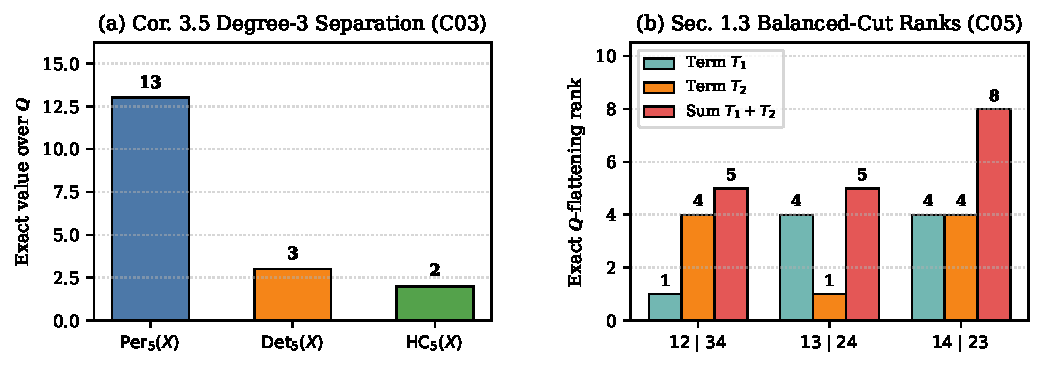
\includegraphics[width=\columnwidth]{figures/fig1_sparse_and_balanced_cuts.pdf}
\caption{(a)~Corollary~3.5 degree-$\le 3$ separation on a 5-vertex 3-regular circulant digraph (\texttt{C03}): $\operatorname{Per}_5=13$, $\operatorname{Det}_5=3$, and $\operatorname{HC}_5=2$ over $\mathbb{Q}$. (b)~Section~1.3 4-row balanced-cut ranks (\texttt{C05}, $q=2$): each summand has rank~$1$ on its own cut, while $T_1+T_2$ achieves ranks $(5,5,8) > q^2=4$ on every balanced cut.}
\label{fig:1}
\end{figure}

\begin{figure}[t]
\centering
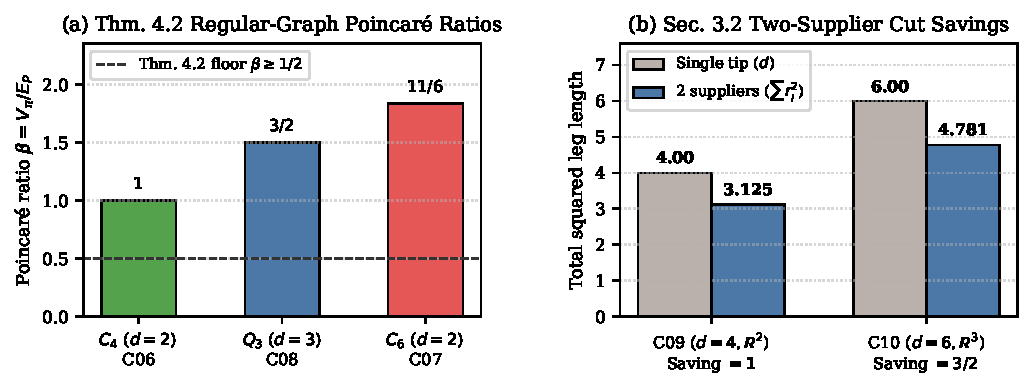
\includegraphics[width=\columnwidth]{figures/fig2_poincare_and_cone_savings.pdf}
\caption{(a)~Exact Poincar\'e ratios $\beta = V_\pi/E_P$ across regular graphs $C_4$ ($1$, \texttt{C06}), $Q_3$ ($3/2$, \texttt{C08}), and $C_6$ ($11/6$, \texttt{C07}), all satisfying Theorem~4.2's floor $\beta \ge 1/2$. (b)~Section~3.2 two-supplier transport squared length $\sum r_i^2$ vs.\ single-tip star $d$ (\texttt{C09}: $25/8 = 3.125 < 4$; \texttt{C10}: $153/32 \approx 4.781 < 6$).}
\label{fig:2}
\end{figure}

\subsection{Worked Hand-Verifiable Arithmetic}
\paragraph{Witness \texttt{C01} \& \texttt{C03} (Lemma~3.4 Gadget \& Degree-3 Separation).}
In \texttt{C01}, Lemma~3.4's $3\times 3$ coupling matrix
\[
A = \begin{pmatrix} \frac{1}{2} & \frac{1}{2} & -\frac{1}{2} \\ -1 & -1 & 1 \\ 1 & 1 & 1 \end{pmatrix}
\]
satisfies $\operatorname{per}(A) = \frac{1}{2}(0) + \frac{1}{2}(0) + (-\frac{1}{2})(-2) = 1$, all four $2\times 2$ permanent minors deleting $(r,c)\in\{0,1\}^2$ equal $(-1)(1)+(1)(1)=0$ or $\frac{1}{2}(1)+(-\frac{1}{2})(1)=0$, and $A_{33}=1$ (also valid over $\mathbb{F}_7$ in \texttt{C02} since $2^{-1}\equiv 4\pmod 7$). In \texttt{C03}, the 3-regular 5-vertex circulant adjacency matrix with shifts $\{0,1,2\}\pmod 5$ gives exact values $\operatorname{Per}_5(X) = 13$, $\operatorname{Det}_5(X) = 3$, and $\operatorname{HC}_5(X) = 2$ over $\mathbb{Q}$ (Fig.~\ref{fig:1}a), while in \texttt{C04} over $\mathbb{F}_2$ the 4-vertex 3-regular circulant yields $\operatorname{Per}_4 = \operatorname{Det}_4 = 1\pmod 2$.

\paragraph{Witness \texttt{C05} \& \texttt{C07} (Balanced Cuts \& Poincar\'e Smoothing).}
In \texttt{C05} ($q=2$, disjoint row alphabets $\{0,1\}$ and $\{2,3\}$), $T_1 = E_{12}(2)\otimes E_{34}(2)$ has flattening ranks $(1,4,4)$ on cuts $(12\mid 34, 13\mid 24, 14\mid 23)$, and $T_2 = E_{13}(2)\otimes E_{24}(2)$ has ranks $(4,1,4)$; because supports are disjoint on every cut, $T_1+T_2$ has exact ranks $(5,5,8)$ (Fig.~\ref{fig:1}b). In \texttt{C07}, the 2-regular 6-cycle $C_6$ with 1D ramp placement $x=(0,1,2,3,2,1)$ has unit edge energy $E_P(x)=1$ and mean $\bar{x}=\frac{3}{2}$, giving variance $\operatorname{Var}(x)=\frac{11}{12}$, pair variance $V_\pi(x)=2\operatorname{Var}(x)=\frac{11}{6}$, and Poincar\'e ratio $\beta=\frac{11}{6}$ (Fig.~\ref{fig:2}a); exact barycentric smoothing at $t=6$ verifies Eq.~(4.1).

\paragraph{Witness \texttt{C09} \& \texttt{C11} (Cone Savings \& Pl\"ucker Minors).}
In \texttt{C09}, the four unit sites $(\pm 1,0),(0,\pm 1)\in\mathbb{R}^2$ have barycenter $0$. On balanced cut $b=(1,0,1,0)$ with suppliers $Z_1=(\frac{1}{4},\frac{1}{4})$ and $Z_0=(-\frac{1}{4},-\frac{1}{4})$, $\|Z_0-Z_1\|^2 = \frac{1}{2}\le 1$, first-order saving is $4\cdot\frac{1}{4}=1$, and at $\tau=\frac{1}{2}$ each leg has squared length $(\frac{7}{8})^2 + (\frac{1}{8})^2 = \frac{25}{32}$, reducing total squared transport from $4$ to $\frac{25}{8}=3.125$ (Fig.~\ref{fig:2}b). In \texttt{C11}, the $2\times 4$ Vandermonde basis $[(1,1,1,1),(1,2,3,4)]$ over $\mathbb{F}_7$ yields $12$ nonzero alternating $2\times 2$ minors with $p_{01}=1, p_{02}=2, p_{03}=3, p_{12}=1, p_{13}=2, p_{23}=1$, satisfying Pl\"ucker $p_{01}p_{23}-p_{02}p_{13}+p_{03}p_{12} = 1 - 4 + 3 = 0\pmod 7$.

\paragraph{Witness \texttt{C13} \& \texttt{C15} (Cartier Residue \& Sec.~19 Contradiction).}
In \texttt{C13} over $\mathbb{F}_5$, the Laurent series $f(t) = 2t^{-6} + t^{-5} + 4t^{-4} + 2t^{-2} + 3t^{-1} + 1 + 4t^2 + 2t^3 + t^4$ has a pole of order~6. The Cartier operator selects exponents $k\equiv 4\pmod 5$ ($k\in\{-6,-1,4\}\mapsto m\in\{-2,-1,0\}$), recovering exact residue $c_{-1}=3$ at $m=-1$ while annihilating $d(g)$ (Fig.~\ref{fig:3}a). In \texttt{C15} over $\mathbb{F}_7$ ($m=3, H^*=1, \Omega=(2,3,1), Z=(4,2,5)$), setting $v=(1,1,2)$ ($v\cdot\Omega = 7\equiv 0\pmod 7$) and $W(H) = Z(H)I + u_H v^T$ with $u_0=(1,2,3), u_1=(3,1,4), u_2=(2,5,1)$ guarantees $W(H)\Omega = Z(H)\Omega$. The diagonalized program counts Eq.~(19.2) are $P = (0, 6, 4)\pmod 7$ (Fig.~\ref{fig:3}b), yielding $\sum_H P(H)\Omega(H) = 0 + 18 + 4 = 22 \equiv 1\pmod 7$ vs.\ $\sum_I Z(I)\Omega(I) = 8 + 6 + 5 = 19 \equiv 5\pmod 7$, whose difference is $1 - 5 \equiv 3 = \Omega(H^*)\not\equiv 0\pmod 7$.

\begin{figure}[t]
\centering
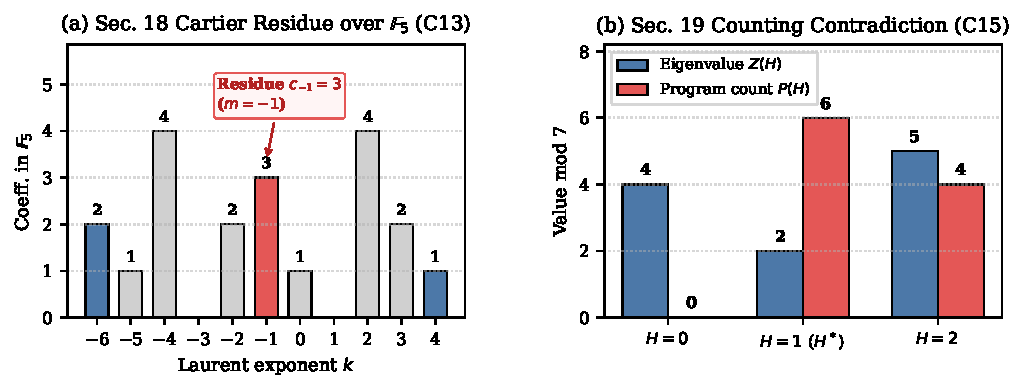
\includegraphics[width=\columnwidth]{figures/fig3_cartier_and_diagonal.pdf}
\caption{(a)~Section~18 Cartier operator over $\mathbb{F}_5$ (\texttt{C13}): selects exponents $k\in\{-6,-1,4\}$ (blue/red) and isolates exact residue $c_{-1}=3$ despite the order-6 pole. (b)~Section~19 Eq.~(19.1)--(19.2) over $\mathbb{F}_7$ (\texttt{C15}): eigenvalue $Z=(4,2,5)$ vs.\ program count $P=(0,6,4)$ yields weighted contradiction gap $\Omega(H^*)=3\not\equiv 0\pmod 7$.}
\label{fig:3}
\end{figure}

\begin{table}[t]
\centering
\scriptsize
\setlength{\tabcolsep}{2.6pt}
\caption{Canonical verified certificate corpus (\texttt{C01}--\texttt{C16}).}
\label{tab:corpus}
\begin{tabular}{@{}clll@{}}
\toprule
ID & Mode / Submode & Key Verified Invariant & Status \\
\midrule
C01 & M1 / Lem.~3.4 ($\mathbb{Q}$) & $\operatorname{per}(A){=}1$, four $2{\times}2$ minors $0$ & PASS \\
C02 & M1 / Lem.~3.4 ($\mathbb{F}_7$) & Odd-char gadget validity ($2^{-1}{=}4$) & PASS \\
C03 & M1 / deg-3 ($\mathbb{Q}$) & $\operatorname{Per}_5{=}13, \operatorname{Det}_5{=}3, \operatorname{HC}_5{=}2$ & PASS \\
C04 & M1 / deg-3 ($\mathbb{F}_2$) & Char-2 $\operatorname{Per}_4{=}\operatorname{Det}_4{=}1$, $\operatorname{HC}_4{=}1$ & PASS \\
C05 & M2 / 4-row cuts & $q{=}2$: sum ranks $(5,5,8) > 4$ & PASS \\
C06 & M2 / Poincar\'e & $C_4$ ($d{=}2$): $\beta{=}1$, Eq.~(4.1) $t{=}4$ & PASS \\
C07 & M2 / Poincar\'e & $C_6$ ($d{=}2$): $\beta{=}11/6$, Eq.~(4.1) $t{=}6$ & PASS \\
C08 & M2 / Poincar\'e & $Q_3$ ($d{=}3$): $\beta{=}3/2$, Eq.~(4.1) $t{=}4$ & PASS \\
C09 & M3 / cone cut & $d{=}4$ ($\mathbb{R}^2$): save $1$, $\sum r_i^2{=}25/8$ & PASS \\
C10 & M3 / cone cut & $d{=}6$ ($\mathbb{R}^3$): save $3/2$, $\sum r_i^2{=}153/32$ & PASS \\
C11 & M3 / minors ($\mathbb{F}_7$) & $k{=}2,n{=}4$: 12 minors, Pl\"ucker $0$ & PASS \\
C12 & M3 / minors ($\mathbb{F}_{11}$) & $k{=}3,n{=}4$: 24 alternating minors & PASS \\
C13 & M4 / Cartier ($\mathbb{F}_5$) & Pole $t^{-6}$, $C(dg){=}0$, res $c_{-1}{=}3$ & PASS \\
C14 & M4 / Cartier ($\mathbb{F}_2$) & Char-2 pole $t^{-4}$, res $c_{-1}{=}1$ & PASS \\
C15 & M4 / Sec.~19 ($\mathbb{F}_7$) & $m{=}3,H^*{=}1$: gap $\Omega(H^*){=}3$ & PASS \\
C16 & M4 / Sec.~19 ($\mathbb{F}_2$) & $m{=}4,H^*{=}2$: char-2 gap $\Omega(H^*){=}1$ & PASS \\
\bottomrule
\end{tabular}
\end{table}

\section{Verification Gates and Reproducibility}
{\raggedright
All artifacts pass five independent gates: (1)~Lean~4.35.0 compilation with 18 constructive theorems, zero warnings, zero custom axioms, and zero \texttt{Classical.choice}; (2)~AST zero-float / zero-division check; (3)~16/16 canonical certificates verified; (4)~42 adversarial forgeries and edge-case checks (60/60 \texttt{pytest} checks total, covering duplicate keys, oversized/deeply nested JSON, \texttt{NaN}/\texttt{Infinity} rejection, non-lowest-terms rationals, $1/p$ pole cancellation attacks over $\mathbb{F}_p$, char-2 permanent gadgets, all-zero matrices, degree-$>3$ digraphs, $q=3$ balanced-cut ranks, odd smoothing steps, asymmetric/non-regular graphs, constant placements, unbalanced cuts, excessive supplier separation, rank-deficient minor bases, pole-free Laurent series, vanishing-derivative $g$, zero $\Omega(H^*)$, and broken Eq.~(19.1) eigenvectors); and (5)~complete SHA-256 integrity manifest (\texttt{MANIFEST.sha256}).\par}

\paragraph{AI Assistance Disclosure.}
This work was produced by Lluis Eriksson using Google Antigravity for Lean~4 theorem drafting, Python exact-verifier engineering, test generation, and \LaTeX{} preparation; all mathematical claims, code, proofs, and verification logs were independently compiled, tested, and reviewed by the author.

\paragraph{Licensing.}
Manuscript and figures are released under \texttt{CC-BY-4.0}; Lean~4 proofs, Python code, and JSON certificates are released under the \texttt{MIT} License.

{\footnotesize\raggedright
\bibliographystyle{plain}
\bibliography{references}
}
\end{document}
